\documentclass[a4paper,11pt]{article}

\usepackage[french]{babel}
\usepackage[T1]{fontenc}
\usepackage[utf8]{inputenc}
\usepackage{graphicx}
%\usepackage{fullpage}

\begin{document}

\title{\textbf{Compte rendu du TP \no 2}\\Opérations morphologiques sur des images}
\author{Thibaut Castanié\\\textit{Master IMAGINA}}
\date{\today}

\maketitle
\thispagestyle{empty}

\newpage 
\section*{Introduction}
Durant le TP, l'image suivante, au format \texttt{.pgm}, a été utilisé pour l'ensemble des opérations :
\begin{center}
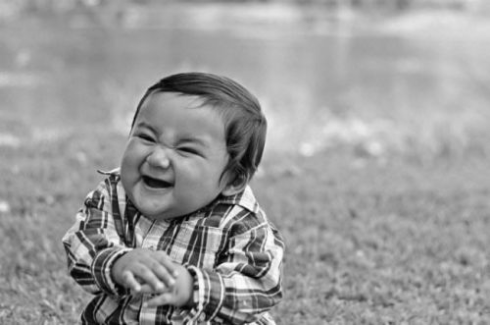
\includegraphics[scale=0.7]{baby.png}
\end{center}
\section{Seuillage d'une image et érosion de l'image binaire}
\subsection{Seuillage}
L'image possède 256 niveaux de gris. Afin de travailler plus efficacement dessus, nous allons devoir définir un seuil tel que tous les pixels inférieurs à celui-ci soient noirs, et les autres soient blancs. Nous obtenons ainsi quatre images avec des seuils différents.
\begin{center}
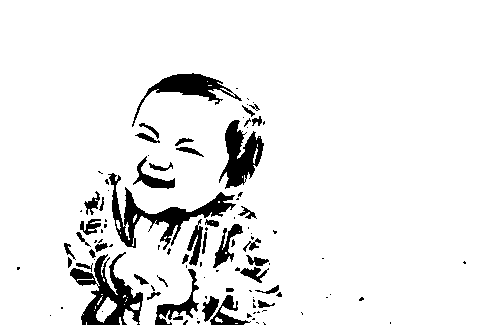
\includegraphics[scale=0.15]{baby2c_90.png}
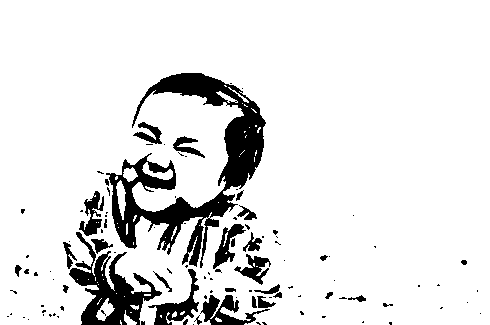
\includegraphics[scale=0.15]{baby2c_110.png}
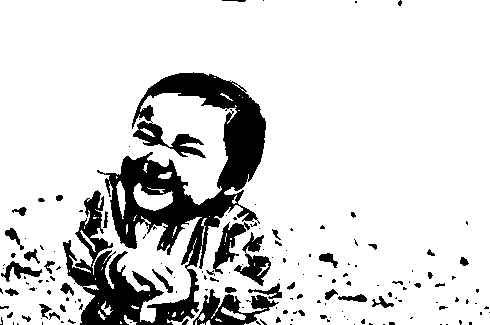
\includegraphics[scale=0.15]{baby2c_128.png}
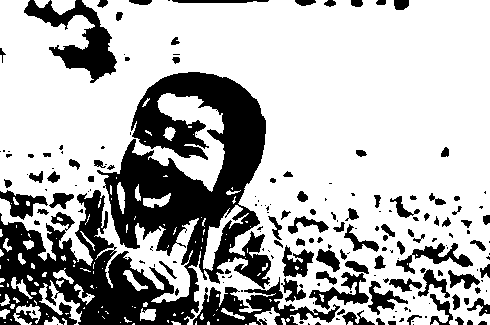
\includegraphics[scale=0.15]{baby2c_150.png}\\
\textit{Valeur seuil 90}
\textit{Valeur seuil 110}
\textit{Valeur seuil 128}
\textit{Valeur seuil 150}
\end{center}L'image ayant pour seuil 128 sera celle que nous utiliserons pour la suite du TP, car l'objet de la scène est en noir tandis que le fond est presque tout blanc.
\begin{center}
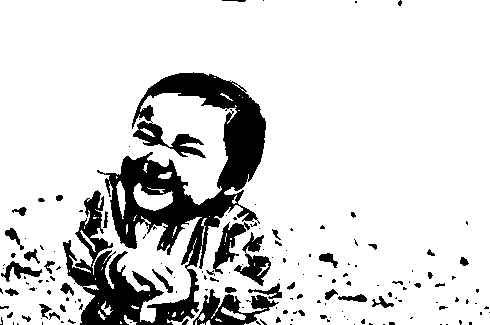
\includegraphics[scale=0.7]{babyo.png}\\
\textit{Image seuillée gardée pour la suite}
\end{center}

\subsection{Érosion}
Une érosion est une opération consistant à réduire d'un pixel "l'épaisseur" de l'objet de la scène. L'algorithme utilisé est simple, à chaque pixel blanc détecté, on change la couleur des 4 pixels voisins en blanc.
\begin{center}
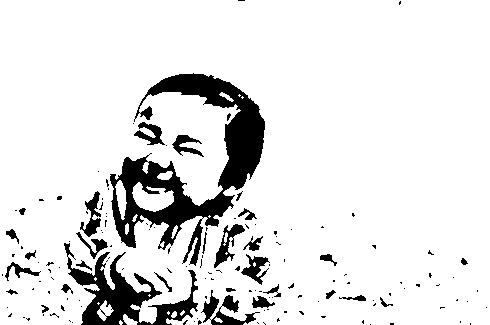
\includegraphics[scale=0.7]{babyerode.png}\\
\textit{Image obtenue après application d'une érosion}
\end{center}

\subsection{Dilatation}
La dilatation est l'inverse de l'érosion, elle fonctionne sur le même principe, sauf que l'objet va prendre du volume. À chaque pixel noir détecté, on change la couleur de ses voisins en noir.
\begin{center}
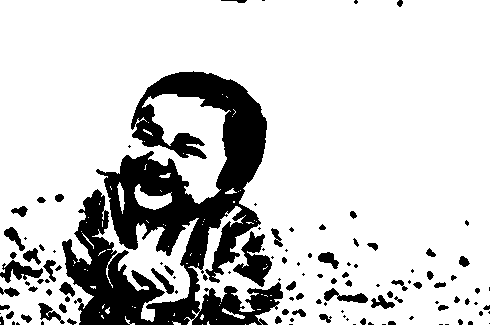
\includegraphics[scale=0.7]{babydilate.png}\\
\textit{Image obtenue après application d'une dilatation}
\end{center}

\newpage
\section{Fermeture et ouverture d'une image de l'image binaire}
\subsection{Fermeture}
Une fermeture permet de boucher les trous présents sur une image en appliquant une dilatation suivie d'une érosion sur une image.
\begin{center}
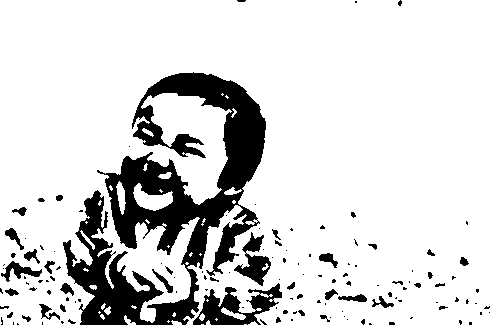
\includegraphics[scale=0.7]{babyferme.png}\\
\textit{Image obtenue après fermeture}
\end{center}
\subsection{Ouverture}
Une fermeture permet de supprimer des points parasites présents sur le fond d'une image en appliquant une ouverture suivie d'une dilatation.
\begin{center}
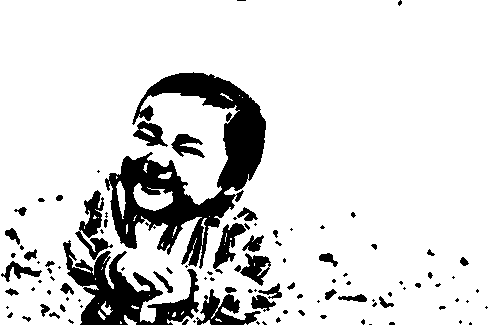
\includegraphics[scale=0.7]{babyouvert.png}\\
\textit{Image obtenue après ouverture}
\end{center}
\subsection{Fermeture puis ouverture}
En appliquant une fermeture suivie d'une ouverture, obtient l'image ci-dessous :
\begin{center}
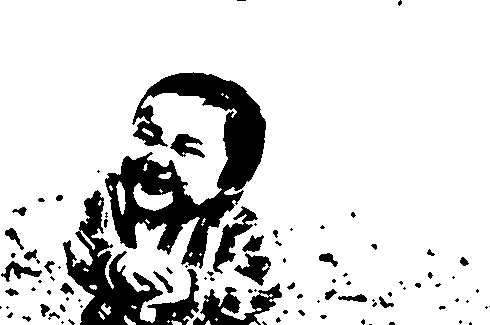
\includegraphics[scale=0.7]{babyfermeouvert.png}\\
\textit{Fermeture-ouverture}
\end{center}
On peut constater que les petits trous on étés bouchés et les plus petits points parasites on disparus par rapport à l'image originale.


\newpage
\subsection{Applications séquentielles}
Afin d'amplifier les effets d'une ouverture et d'une ouverture, nous allons appliquer les opérations d'érosion et de dilatation les unes à la suite des autres.\\
Dans un premier temps, nous effectuerons trois dilatations, suivies de six érosions, puis trois dilatations à nouveau.
\begin{center}
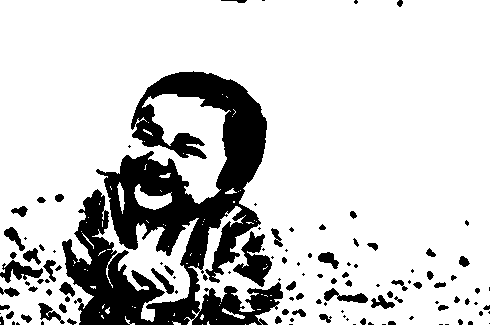
\includegraphics[scale=0.22]{babyd1.png}
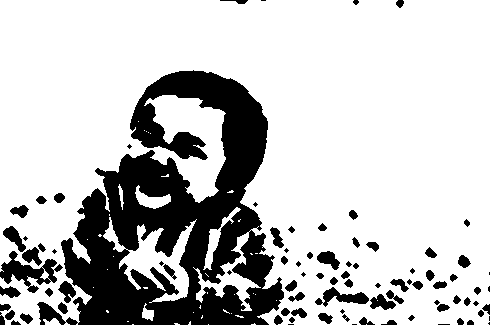
\includegraphics[scale=0.22]{babyd2.png}
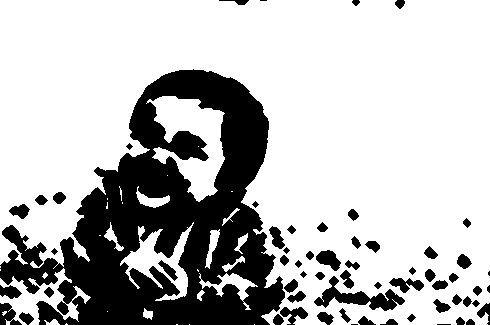
\includegraphics[scale=0.22]{babyd3.png}\\
\textit{Trois dilatations...}
\\
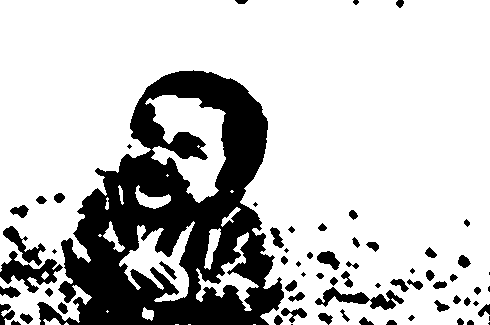
\includegraphics[scale=0.22]{babyd3e1.png}
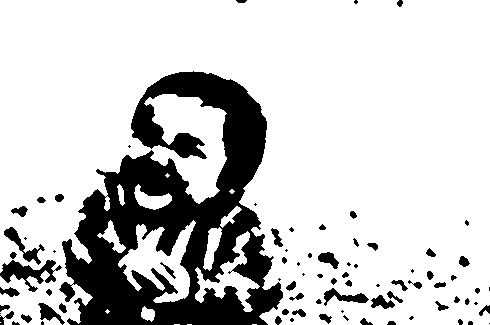
\includegraphics[scale=0.22]{babyd3e2.png}
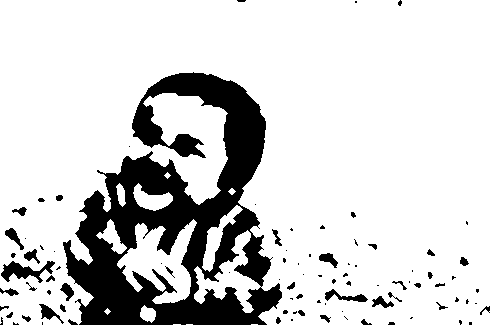
\includegraphics[scale=0.22]{babyd3e3.png}\\
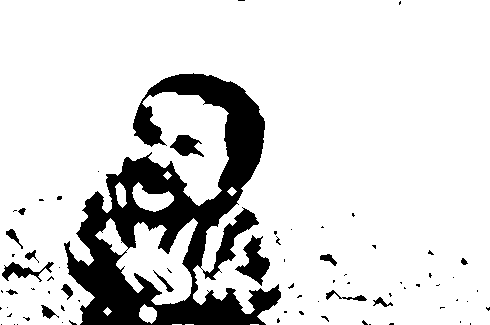
\includegraphics[scale=0.22]{babyd3e4.png}
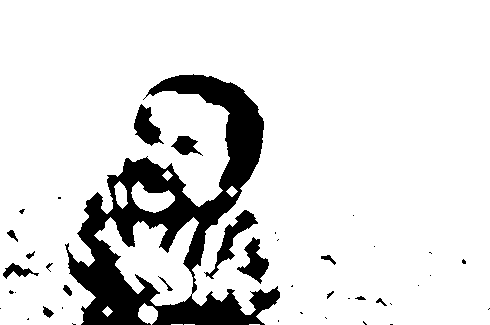
\includegraphics[scale=0.22]{babyd3e5.png}
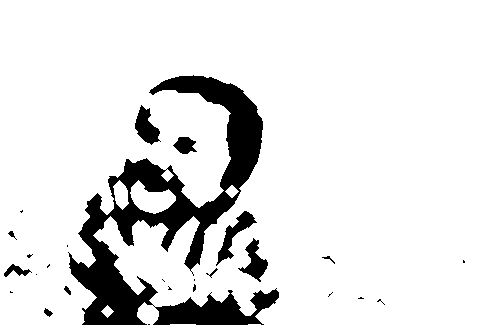
\includegraphics[scale=0.22]{babyd3e6.png}\\
\textit{...suivies de six érosions...}
\\
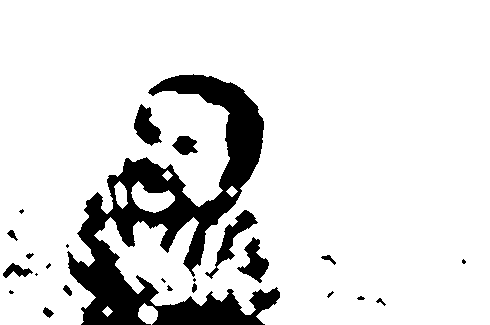
\includegraphics[scale=0.22]{babyd3e6d1.png}
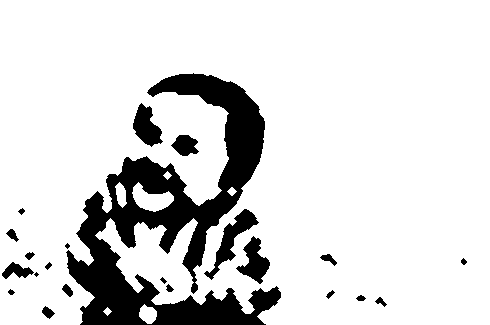
\includegraphics[scale=0.22]{babyd3e6d2.png}
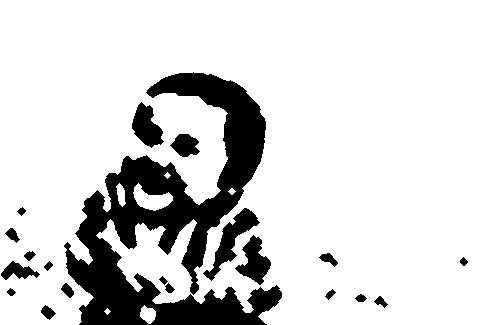
\includegraphics[scale=0.22]{babyd3e6d3.png}\\
\textit{...puis encore trois dilatations}
\\
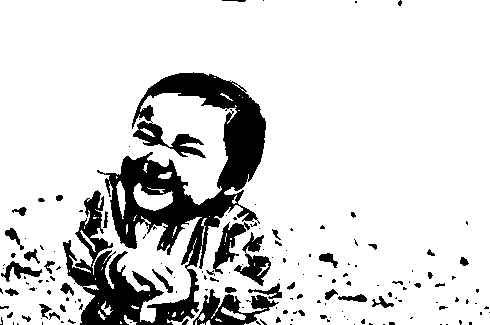
\includegraphics[scale=0.35]{babyo.png}
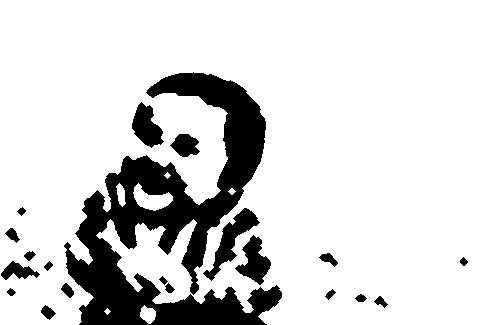
\includegraphics[scale=0.35]{babyd3e6d3.png}\\
\textit{Avant / Après}
\end{center}

\section{Segmentation d'une image}
En utilisant l'image seuillée, ainsi que l'image dilatée une fois, nous pouvons obtenir le contour de notre objet, en supposant que celui ci soit en noir. Il suffit de faire la différence entre l'image dilatée et l'image seuillée. Seuls les pixels noirs commun aux deux images en entrée seront conservés. Sur notre image, on obtient le résultat suivant.
\begin{center}
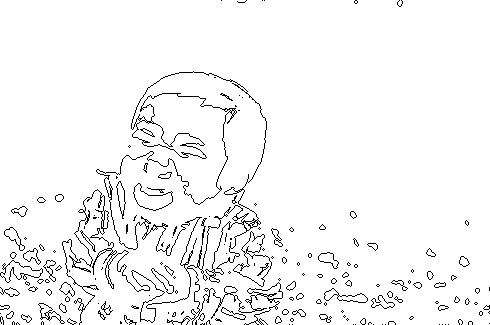
\includegraphics[scale=0.7]{babyDiff.png}\\
\textit{Contour de l'objet}
\end{center}

\section{Extension aux images en niveaux de gris, puis en couleurs}
En essayant d'appliquer la méthode d'érosion et de dilatation sur une image non seuillée, on obtient des résultats plutôt moches. En effet, dans l'algorithme de ces opérations, on part du principe qu'il y a peu de couleurs et que chacune d'entre elle représente une forme de la scène. On utilise donc la couleur du pixel voisin pour éroder ou ouvrir. Sur une image non seuillée, on obtient ainsi une sorte de bordure autour de notre objet. Cela est dû au fait qu'on ne peut pas deviner les motifs formés par les pixels de l'arrière-plan ou de l'objet.
\begin{center}
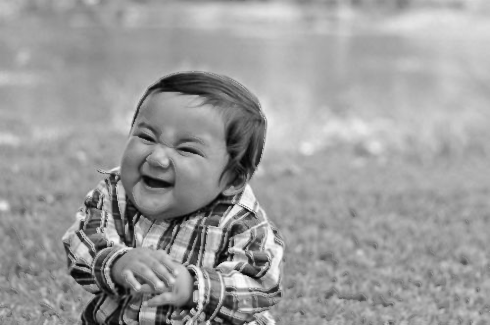
\includegraphics[scale=0.35]{babyerodeg1.png}
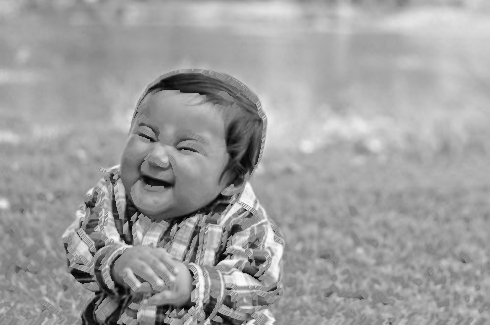
\includegraphics[scale=0.35]{babyerodeg3.png}\\
\textit{Une, puis trois érosions successives}
\\
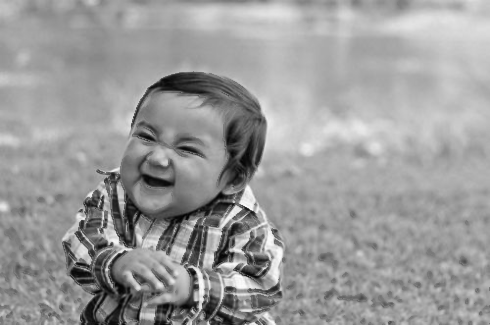
\includegraphics[scale=0.35]{babydilateg1.png}
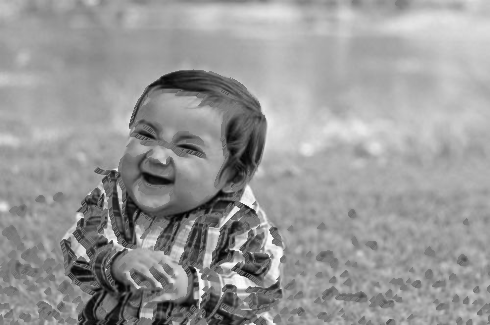
\includegraphics[scale=0.35]{babydilateg3.png}\\
\textit{Une, puis trois dilatations successives}
\end{center}
Après seuillage d'une image couleur, au format \texttt{ppm}, on obtient néanmoins les résultats suivants :
\begin{center}
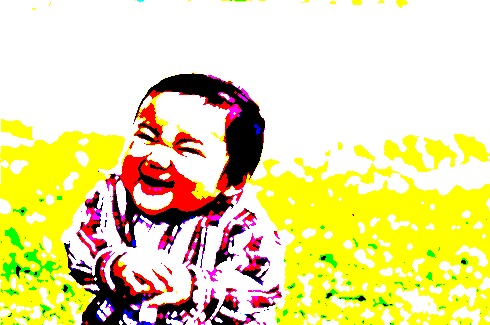
\includegraphics[scale=0.7]{babyerodec1.png}\\
\textit{Érosion}\\
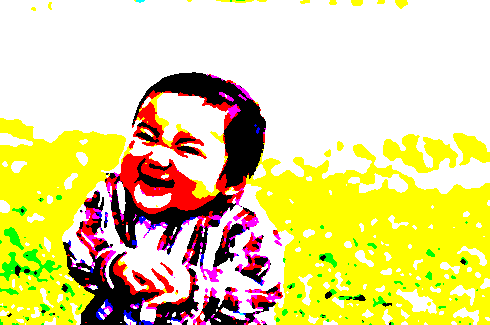
\includegraphics[scale=0.7]{babydilatecL.png}\\
\textit{Dilatation}
\end{center}


\end{document}